\documentclass{rapportECL}
\usepackage{lipsum}
\usepackage{biblatex} %Imports biblatex package
\addbibresource{bibliotheque.bib}

\title{Rapport ECL - Template} %Titre du fichier

\begin{document}

%----------- Informations du rapport ---------

\titre{Un Langage "Pur" pour Web Assembly} %Titre du fichier .pdf
\UE{PSTL} %Nom de la UE

\enseignant{Frédéric \textsc{Peschanski}} %Nom de l'enseignant

\eleves{Lucas \textssc{Fumard} \\
	Lauryn \textsc{Pierre} \\
	Saïd Mohammad \textsc{ZUHAIR} } %Nom des élèves

%----------- Initialisation -------------------

\fairemarges %Afficher les marges
\fairepagedegarde %Créer la page de garde
\tabledematieres %Créer la table de matières

%------------ Corps du rapport ----------------
\section{Introduction}
Le but de notre projet est de concevoir un langage 100 $\%$ fonctionnel et “pur” pour WebAssembly en 
se basant sur cet article\cite{ullrich_counting_2020}(fourni). L'article défini un langage fonctionnel dont la gestion de la mémoire se fait par 
un mécanisme de comptage de références.
WebAssembly\cite{noauthor_webassembly_nodate} ou Wasm définit un format de code binaire portable
et un langage de type assembleur\cite{noauthor_webassembly_2023}. Tous les principaux navigateurs peuvent exécuter des programmes WebAssembly. 
Des langages comme C, C++, Rust, Go et bien d'autres peuvent être compilés en WebAssembly. 

\section{WebAsssembly}

JavaScript est le seul langage de programmation native au Web. 
Pour de nombreuses raisons, JavaScript n’est pas idéal pour être une cible de compilation efficace pour les langages de bas niveau tels que C/C++ et Rust. 
WebAssembly a plusieurs objectifs\cite{haas_bringing_2017}. Être sûre, les programmes WebAssembly sont isolées de leur environnement hôte. 
WebAssembly est conçu pour être lié à aucun runtime ou langages de programmation, de sorte qu'il peut être exécuté sur n'importe quel 
appareil qui le prend en charge et d’avoir le même comportement. 
Ce qui le rend intéressant pour la création d'applications multiplateformes.
Les programmes pouvant être exécutées sur des ordinateurs de bureau, des appareils mobiles, et même des serveurs. 
WebAssembly fonctionne avec les technologies Web existants, par exemple JavaScript, CSS, et HTML.
WebAssembly est un langage bytecode portable de bas niveau pris en charge par les principaux navigateurs Web. 
Les utilisations de WebAssembly ne se limitent pas qu'au Web, il y a aussi un intérêt pour l'Internet des Objets, les serveurs, les systèmes embarqués.
\par WebAssembly a un format texte (.wat) et un format binaire (.wasm). 
WebAssembly peut être exécuté dans différents environnements, tels que les serveurs, les navigateurs web ou les applications. 
Dans les navigateurs web, WebAssembly est exécuté en même temps que le code JavaScript. 
Pour les serveurs, WebAssembly est exécuté en utilisant des runtimes tels que Node.js. 
Plusieurs compilateurs ont été développés pour WebAssembly\cite{noauthor_wabt_2023,noauthor_wasm3_2023,noauthor_wasmer_nodate,noauthor_wasmtime_nodate}. 
Wasmer\cite{noauthor_wasmer_nodate} et wasmtime\cite{noauthor_wasmtime_nodate} sont les plus connues. 
Ils utilisent tous les deux la technique de la compilation à la volée. Wasmtime est développé en collaboration supervisée par la fondation Mozilla. 
Alors que wasmer est développé par une entreprise privée. 
Dans le cadre de notre projet, on utilise wabt\cite{noauthor_wabt_2023} pour compiler et on exécute le compilé à l’aide de Node.js\cite{noauthor_nodejs_nodate}. 
\par Les programmes sont composés d'un ou plusieurs modules. Un module contient la définition des fonctions, variables globales. 
Les définitions peuvent être importées ou exportées.
Ils interagissent avec l’environnement à l’aide d’import et d’export explicites. 
Un module doit être validé avant l’exécution pour s’assurer qu’il est bien typé et sûr d’exécuter. 
WebAssembly possède un système de type statique centré autour de quatre valeurs :  i32, i64, f32 et f64. 
Qui désignent les nombres entiers de 32 bits et 64 bits et les flottants de 32 et 64 bits.  
La spécification officielle de Wasm comprend une sémantique formelle pour le langage, 
avec une déclaration précise de la propriété de solidité des types prévue. 
Elle a d'abord été publiée dans un premier projet en 2017, puis dans la norme officielle, appelée WebAssembly 1.0 (Wasm 1.0), en 2019.
\par La mémoire d’un programme Wasm repose sur le modèle de mémoire linéaire\cite{haas_bringing_2017}. 
La mémoire linéaire est un tampon continu d'octets non signés  que JavaScript et Wasm peuvent lire et modifier de manière synchrone. 
Au cours de l’exécution, l’espace mémoire peut grandir. 

\begin{figure}[ht]
	\centering
	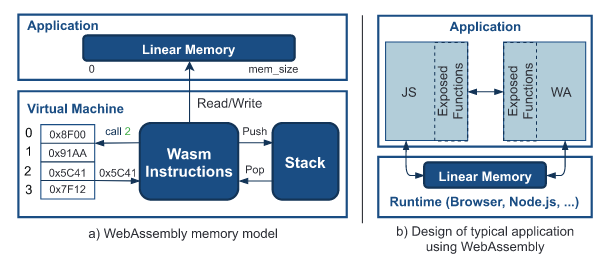
\includegraphics[scale=0.65]{logos/model_memory_wasm.png}	
	\caption{WebAssembly Architecture \cite{noauthor_wasmati_nodate}}
\end{figure}
\section{Cahier des charges}
Les tâches que nous avons identifiées sont les suivantes :

- Analyser le fonctionnement de WASM et étudier son écosystème.

- Programmer un parseur qui puisse lire le langage pur tel que défini dans l'article\cite{ullrich_counting_2020}

- Programmer un interpréteur en Rust du langage selon les sémantiques du langage pur

- Définir quelques tests unitaires couvrant les sémantiques définies dans l'article

- Ajouter la gestion des instructions \verb|inc|, \verb|dec|, \verb|reset|, \verb|reuse|

- Programmer un compilateur du langage agrandi vers WASM

\section{Tâches Réalisées}

\subsection{Lecture de l'article}
Le langage fonctionnel décrit dans l'article\cite{ullrich_counting_2020} alloue ses constructeurs dans la pile et manipule des 
adresses vers ces emplacements mémoire alloués. Il est donc primordial d'avoir un système d'allocation et réutilisation de 
mémoire performant afin d'éviter les fuites mémoires et un temps d'exécution faible.

Le système de la gestion de la mémoire par comptage de référence est bien plus vieux que des systèmes par garbage collector, 
mais aussi plus efficaces\cite{ullrich_counting_2020}. Cependant, la gestion de mémoire comptage de références ne fonctionne que si 
il n'est pas possible de créer de cycle de référence. 
C'est pourquoi les garbage collector ne sont plus utilisés de nos jours.

Les auteurs de l'article\cite{ullrich_counting_2020} ont créé un langage fonctionnel dans lequel les cycles de références 
sont impossibles afin d'implémenter un système de gestion de mémoire par comptage de référence et d'obtenir un langage fonctionnel 
dont l'exécution est optimisée. Ils définissent un langage source $\lambda_{pure}$. 
Qui, après une étape de compilation, deviendra $\lambda_{RC}$, notre langage de destination.
$\lambda_{RC}$ est une extension de $\lambda_{pure}$ auquel on a ajouté les instructions de gestion de la mémoire : 
\verb|inc|, \verb|dec|, \verb|reset|, \verb|reuse|.
Notre interpréteur implémentera $\lambda_{pure}$.

\begin{figure}[hbt!]
	\centering
	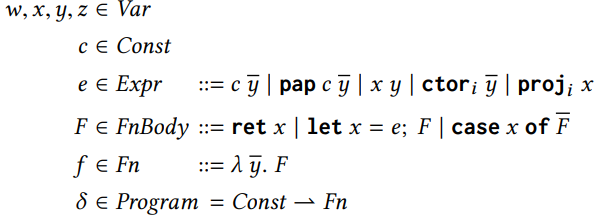
\includegraphics[scale=0.65]{logos/grammaire.png}
	\caption{Grammaire du langage source $\lambda_{pure}$}
	\label{fig:grammaire pure}
\end{figure}
\FloatBarrier

\begin{figure}[hbt!]
	\centering
	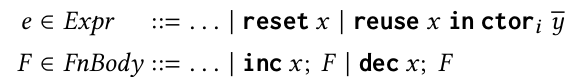
\includegraphics[scale=0.40]{logos/grammaire_RC.png}
	\caption{Grammaire du langage $\lambda_{RC}$}
	\label{fig:grammaire RC}
\end{figure}
\FloatBarrier 

\subsection{Parser/reader}
Concernant la grammaire du langage, nous reprenons celle qui est définie dans la section 3 de l'article et retranscrit dans la Figure ~\ref{fig:grammaire pure}.


Notre reader utilise la bibliothèque Chumsky\cite{zesterer_chumsky_nodate}, ainsi, nous ne pouvons pas stoker les noms définis 
variables, ce qui nous empêche de distinguer directement les constantes des variables.

\subsection{Interpréteur}

Afin d'implémenter un interpréteur du langage décrit, il nous a d'abord fallu implémenter les structures permettant d'accéder à la mémoire, 
dont les structures du tas et de la pile (\verb|Heap| et \verb|Ctxt|).

\begin{figure}[hbt!]
	\centering
	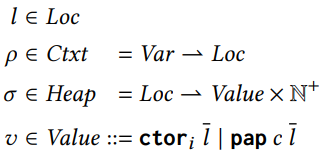
\includegraphics[scale=0.65]{logos/figure_strutures_interpreteur.png}
	\caption{Structures de gestion de la mémoire}
\end{figure}
\FloatBarrier 


\verb|Loc| est l'adresse de la case mémoire allouée pour la valeur dans le tas. C'est la valeur de retour de toutes les sémantiques 
du langage, tel que définies dans la figure 1 de l'article\cite{ullrich_counting_2020}.
Contrairement à l'article, nous avons choisi de ne pas retourner un nouveau tas à chaque fois, mais de garder un même tas que 
l'on modifie par effet de bord. 

Nous avons testé cet interpréteur en créant plusieurs tests unitaires sur les sémantiques, mais aussi quelques programmes simples, 
tels que le calcul de fibonacci, ou le programme \verb|swap| défini à la page 5 de l'article\cite{ullrich_counting_2020}.

WebAssembly ne possède que des types numériques (i32, f32, i64, f64) ainsi, il est compliqué d'implémenter les applications partielles. 
Ainsi, nous nous réservons le droit de ne pas les implémenter.

Afin d'implémenter le tas en WebAssembly, nous utilisons une \verb|Table| qui nous permet de définir une table dans la mémoire que 
nous pouvons manipuler de WebAssembly ainsi que de JavaScript. Cette table nous permettra de réaliser des diagnostics ainsi que 
des évaluations de l'empreinte mémoire.
Nous avons commencé à définir le schéma du tas du code compilé :
La case mémoire 0 est réservée pour indiquer le prochain espace mémoire libre.
Ensuite, chaque constructeur suit le format suivant : \verb|<type> <nb_ref> <args>|. Ainsi, un constructeur \verb|FALSE| référencé 
deux fois est représenté sous la forme "0 2" dans la mémoire. Un entier 10 référencé 3 fois sous la forme "4 3 10".

\section{Tâches Restantes}

Il nous faut choisir un schéma de mémoire pour les objets dans la mémoire.
Il nous faut implémenter \verb|inc|, \verb|dec|, \verb|reset|, \verb|reuse|.
Il nous faut faire le compilateur en WASM

WASM n'a qu'un seul type de variable : les nombres (entiers ou flottant, 32 bit ou 64 bit). 
Ainsi, il faut que l'on interprète différemment ces nombres selon le contexte dans lequel on les prend. 
Dans la mémoire, nos constructeurs et applications partielles seront stockés sous la forme \verb|<type> <nombre de références> <arguments>|. 
Par exemple, une application partielle est sous la forme \verb|6 1 7 2 12 13| où 6 est le type "application partielle", 
1 est le nombre de références à cette application partielle, 
7 est l'identifiant de la fonction à appeler (dans l'interpréteur, on utilise des \verb|string|), 
2 est le nombre d'arguments fixés et 12 et 13 sont les arguments fixés.

Dû à la difficulté d'une telle tâche, nous laissons l'implémentation des applications partielles pour plus tard.

\printbibliography
\end{document}